
%(BEGIN_QUESTION)
% Copyright 2009, Tony R. Kuphaldt, released under the Creative Commons Attribution License (v 1.0)
% This means you may do almost anything with this work of mine, so long as you give me proper credit

Read and outline the ``LRV and URV Settings, Digital Trim (Digital Transmitters)'' section of the ``Instrument Calibration'' chapter in your {\it Lessons In Industrial Instrumentation} textbook.  Note the page numbers where important illustrations, photographs, equations, tables, and other relevant details are found.  Prepare to thoughtfully discuss with your instructor and classmates the concepts and examples explored in this reading.

\underbar{file i03905}
%(END_QUESTION)





%(BEGIN_ANSWER)


%(END_ANSWER)





%(BEGIN_NOTES)

Digital transmitters with analog (4-20 mA) outputs have calibration adjustments for sensing (ADC) as well as output (DAC), and also range settings in the microprocessor determining the desired input-to-output function.  LRV and URV range parameters do not constitute transmitter calibration!  Only by comparing the real analog input and output of an instrument against a trusted standard can we really check the instrument's calibration.  Adjustments may be made to the ADC and DAC by performing ``digital trims'' on the instrument.  

\vskip 10pt

Comparing the transmitter's reported input and output values (on a communicator device) against trusted analog standards connected to the transmitters input and output is the only way to check the actual calibration of a digital transmitter.  A sensor trim error shows up as a disagreement between the real analog input value versus the communicator's reported PV value.  An output trim error shows up as a disagreement between the real analog output value and the communicator's reported output value.

\vskip 10pt

Digital transmitters may be re-ranged simply by entering new LRV and/or URV values, without need for complete recalibration of the ADC or DAC.  Analog transmitters, by contrast, cannot be re-ranged without re-calibration.









\vskip 20pt \vbox{\hrule \hbox{\strut \vrule{} {\bf Suggestions for Socratic discussion} \vrule} \hrule}

\begin{itemize}
\item{} Explain how {\it calibration} (trimming) and {\it ranging} are not the same things.
\item{} Suppose an instrument technician tells you they used a HART communicator to calibrate the LRV and URV for a pressure transmitter.  What is wrong with this statement, and what should the technician do in order to actually calibrate the instrument?
\item{} Explain how {\it calibration} (trimming) and {\it ranging} are separate activities for a smart transmitter, but identical activities for an analog transmitter.
\item{} Explain how we can identify a sensor trim error in a smart transmitter, using a HART communicator to read its internal register values.
\item{} Explain how we can identify an output trim error in a smart transmitter, using a HART communicator to read its internal register values.
\item{} Modify the figures in the block diagram of a smart transmitter to show what a DAC calibration error (output trim error) would look like, as opposed to the sensor calibration error that's shown.
\item{} Under what circumstances might a technician need to re-calibrate a transmitter?
\item{} Under what circumstances might a technician need to re-range a transmitter?
\end{itemize}

















\vfil \eject

\noindent
{\bf Prep Quiz:}

Identify the nature of the calibration error in this HART pressure transmitter, given the information shown in this illustration:

$$\includegraphics[width=15.5cm]{i03905x01.eps}$$

\begin{itemize}
\item{} Incorrect range values (LRV/URV)
\vskip 5pt 
\item{} Output (DAC) calibration error
\vskip 5pt 
\item{} Inadequate power supply voltage
\vskip 5pt 
\item{} Input (sensor or ADC) calibration error
\vskip 5pt 
\item{} Inadequate air supply pressure
\vskip 5pt 
\item{} Loop resistor value incorrect
\end{itemize}


\vfil \eject

\noindent
{\bf Prep Quiz:}

Identify the nature of the calibration error in this HART pressure transmitter, given the information shown in this illustration:

$$\includegraphics[width=15.5cm]{i03905x02.eps}$$

\begin{itemize}
\item{} Incorrect range values (LRV/URV)
\vskip 5pt 
\item{} Output (DAC) calibration error
\vskip 5pt 
\item{} Inadequate power supply voltage
\vskip 5pt 
\item{} Input (sensor or ADC) calibration error
\vskip 5pt 
\item{} Inadequate air supply pressure
\vskip 5pt 
\item{} Loop resistor value incorrect
\end{itemize}


%INDEX% Calibration, smart transmitter: digital trim
%INDEX% Reading assignment: Lessons In Industrial Instrumentation, Instrument Calibration

%(END_NOTES)


